\chapter{خلاصه‌ای از توابع پایه شعاعی} \label{se:rbf}

این فصل، مروری بر توابع پایه شعاعی و خواص آن می‌باشد. تعریف توابع پایه شعاعی به همراه خواص 
\index{درونیاب}
درونیاب ایجاد شده توسط این نوع توابع برای نقاط پراکنده مورد بحث قرار می‌گیرد. همچنین خلاصه‌ای از جزییات محاسباتی و نظری تابع درونیاب ایجاد شده بیا‌ن می‌شود.

توابع دو یا سه ضابطه‌ای را می‌توان بصورت زیر ایجاد کرد.

\begin{equation}
	f(x)=\left\{
	\begin{array}{ll}
		\exp{x} &\text{if}~ x<0 \\
		x^2 & \text{if}~0\leq x<2 \\
		x^3+x^2+1 &\text{if}~2\leq x<6
	\end{array}\right.
\end{equation}


\section{ایجاد محیط‌های نگارشی ویژه}

\begin{definition}
	نمونه تعریف: برای ایجاد محیط تعریف به همین ترتیب عمل شود.
\end{definition}

\begin{lem}
	نمونه لم: برای ایجاد محیط لم به همین ترتیب عمل شود.
\end{lem}

\begin{theo}
	نمونه قضیه: برای ایجاد محیط قضیه به همین ترتیب عمل شود.
\end{theo}

\begin{example}
	نمونه مثال: برای ایجاد محیط مثال به همین ترتیب عمل شود.
\end{example}

%
%
\section{توابع پایه شعاعی}

\begin{definition}
	تابع
	$f:\mathbb{R}^d\rightarrow\mathbb{R}$ 
	یک تابع شعاعی نامیده می‌شود هرگاه یک تابع یک متغیره 
	
	$\phi:[0,\infty)\rightarrow\mathbb{R}$ 
	موجود باشد بطوریکه 
	\begin{eqnarray}
		f(x)=\phi(\|x\|),\quad x\in \mathbb{R}^d\label{eq:radial}
	\end{eqnarray}
	که 
	$\|.\|$,
	نرم اقلیدسی می‌باشد.
\end{definition}
%
\begin{lem}
	به ازای هر مجموعه از نقاط مجزای
	$x_1,\ldots,x_N\in\mathbb{R}^d$,
	تابع پیوسته
	$\phi:\mathbb{R}^d\rightarrow\mathbb{R}$ 
	تابع معین مثبت شرطی  از مرتبه
	$m$
	نامیده می‌شود هر گاه ضرایب
	$\lambda_1,\ldots,\lambda_N$
	در رابطه زیر صدق کنند
	\begin{equation*}
		\sum_{i=1}^{N}\lambda_ip(x_i)=0,
	\end{equation*}
	که در آن
	$p$
	همه چند جمله‌ای‌های از درجه کوچکتر و مساوی
	$m$
	بوده و داریم:
	\begin{equation*}
		\sum_{i=1}^{N}\sum_{j=1}^{N}\lambda_i\lambda_j\phi(\|x_i-x_j\|)>0.
	\end{equation*}
\end{lem}

توابع پایه شعاعی معین مثبت شرطی از مرتبه صفر را توابع پایه شعاعی معین مثبت اکید می‌نامند. توابع گاوسی و مالتی کوادریک معکوس نمونه‌هایی از توابع پایه شعاعی معین مثبت اکید هستند.

پرامتر پهنا،
$\varepsilon$
نقش مهمی در نرخ همگرایی تقریب‌ها و عدد حالت ماتریس تولید شده دارد
\citep{Wendland,Fasshauer}.

توابع پایه شعاعی را می‌توان به دو دسته کلی تقسیم بندی کرد: توابع بصورت نامتناهی هموار و شامل پرامتر آزاد (پارامتر پهنا)
\index{پارامتر پهنا}
و  توابع بصورت قطعه‌ای هموار و فاقد پارامتر آزاد. باید توجه کرد که تعدادی از خواص توابع هموار تفاوت زیادی با توابع پایه‌ای قطعه‌ای  هموار دارد. به عنوان مثال نرخ همگرایی توابع پایه‌ای هموار برای دسته‌ای از توابع مورد درونیابی نمایی است درحالی که نرخ همگرایی توابع پایه‌ای قطعه‌ای هموار برای همه توابع از نوع چندجمله‌ای است. لازم به ذکر است که  بدحالتی ماتریس متناظر با توابع هموار در مقایسه با توابع قطعه‌ای هموار بیشتر است. در این رساله، استفاده از توابع پایه‌ای هموار مورد توجه و تمرکز قرار گرفته است.

رده دیگری از توابع پایه‌ای که نتیجه تحقیقات انجام شده در 
\citep{Wendland,Wu} 
می‌باشند را توابع پایه شعاعی با تکیه گاه فشرده می‌نامند. ایده اصلی این نوع توابع استفاده از چندجمله‌ای‌ها   بعنوان تابعی از 
$\|.\|$
با تکیه‌گاهی روی گوی واحد است. به ازای هر
$d$
کوچکتر یا مساوی مقدار ثابت
$d_0$
توابع پایه شعاعی با تکیه‌گاه فشرده در فضای
$\mathbb{R}^d$
معین مثبت است. تعریف پایه‌ای توابع با تکیه‌گاه فشرده
$\phi_{l,k}$
بصورت 
\begin{equation}
	\phi_{l,k}(r)=(1-r)^n_+p(r)\quad k\geq1,\label{eq:compact}
\end{equation}
است که در آن 
$r=\|.\|$, $(1-r)_+=\max\{0,(1-r)\}$
و
$l=\lfloor\frac{d}{2}\rfloor+k+1$
بعد فضاست. در معادله
(\ref{eq:compact}) $p(r)$
یک چند جمله‌ای و 
$\phi_{l,k}$
دارای مشتقات پیوسته تا مرتبه
$2k$
است. توابع پایه شعاعی متداول وندلند
\LTRfootnote{Wendland} 
به ازای 
$d=3$
با تکیه‌گاه فشرده در جدول 
\ref{tab:crbf}
معرفی شده است. لازم به ذکر است که توابع معرفی شده در جدول 
\ref{tab:crbf}
را می توان با تغییر مقیاس متغیر
$r$
با
$\frac{r}{\sigma}$
به توابع با تکیه‌گاهی در
$[0,\sigma]$
تغییر داد. نمودار تعدادی از توابع پایه‌ای با پارامتر پهنای متفاوت در شکل
\ref{fig:rbf}
نشان داده شده است.
\begin{table}
	\caption{ جواب تقریبی اختیار فروش امریکایی با دو دارایی پایه ناهمبسته با توزیع یکنواخت نقاط به ازای
		$\varepsilon=1.5$}
	\label{tab:crbf}
	\vspace{-0.3cm}\begin{eqnarray*}\hspace{-.5cm}\begin{array}{l l}
			\hline {\rm \text{توابع پایه شعاعی} }
			&\hspace{3cm} {\rm \text{مرتبه همواری}} \\
			\hline
			\phi(r)=(1-r)_+^2                                      &\hspace{3cm} C^0         \\
			\phi(r)=(1-r)_+^4(4r+1)                                &\hspace{3cm} C^2         \\
			\phi(r)=(1-r)_+^6(35r^2+18r+3)                         &\hspace{3cm} C^4        \\
			\phi(r)=(1-r)_+^8(32r^3+25r^2+8r+1)                    &\hspace{3cm} C^6        \\
			\hline
	\end{array}\end{eqnarray*}
\end{table}
%
%
\begin{figure}
	\centerline{
		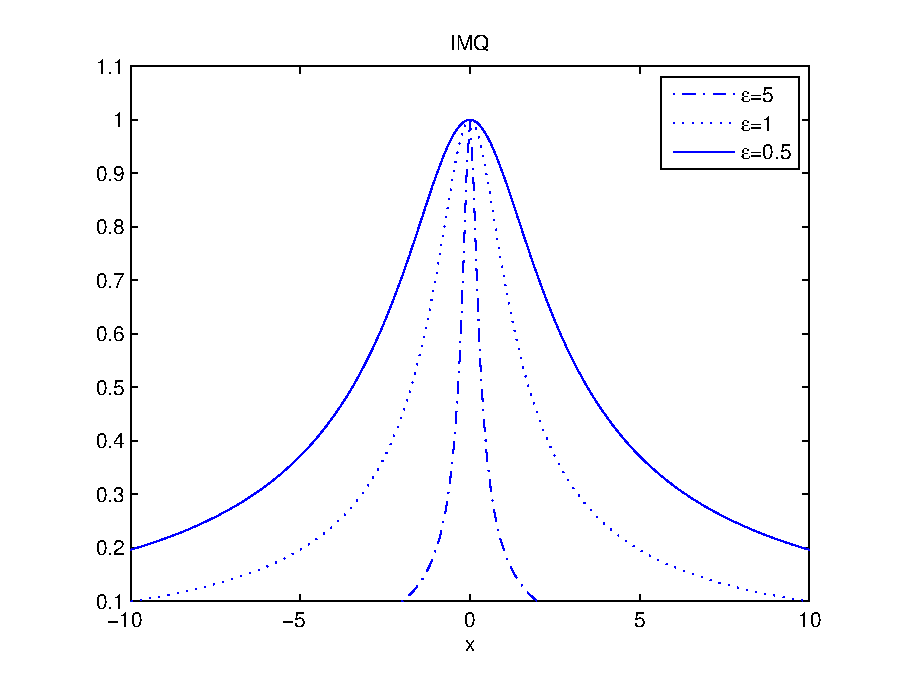
\includegraphics[height=5.5cm]{IMQ.eps}
		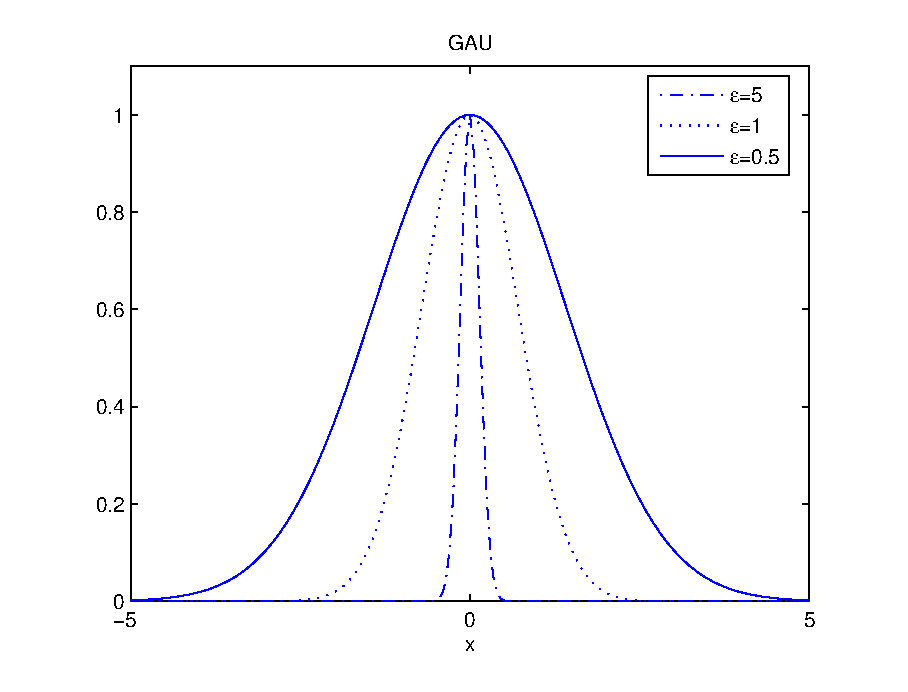
\includegraphics[height=5.5cm]{Gaussian.eps}}
	\centerline{
		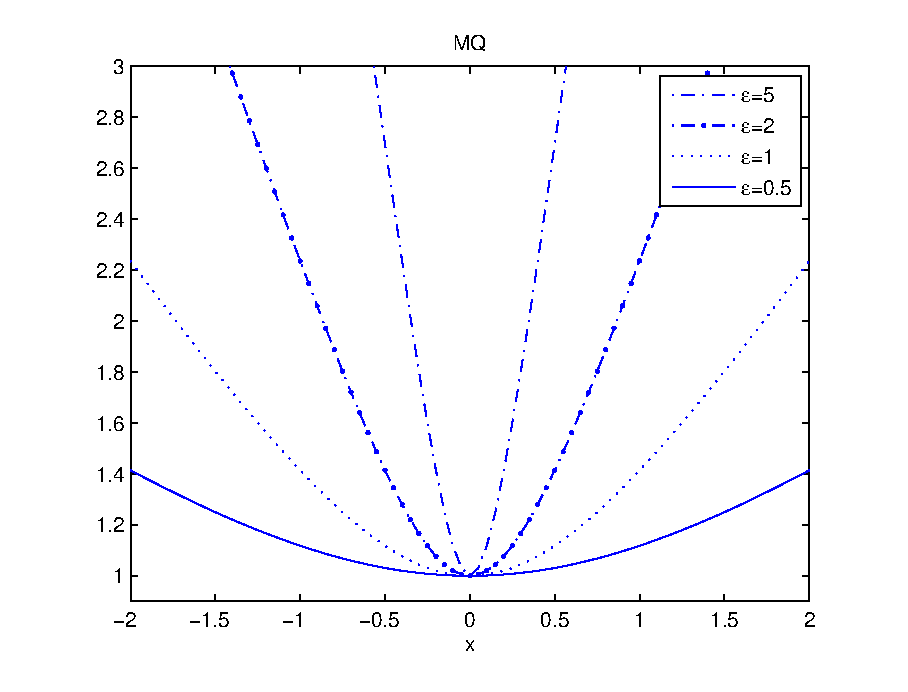
\includegraphics[height=5.5cm]{MQ.eps}
		\includegraphics[height=5.5cm]{compact.eps}} 
	\caption{
		نمودار یک بعدی تعدادی از توابع پایه شعاعی با پارامتر پهناهای متفاوت}
	\label{fig:rbf}
\end{figure}
%


\section{درونیابی با توابع پایه شعاعی}
نقطه‌های متمایز 
$x_1,\ldots,x_N\in\mathbb{R}^d$
و مقدار تابع
$u(x_1),\ldots,u(x_N)$
متناظر با آن نقاط مفروض است. مساله استاندارد درونیابی با استفاده از توابع پایه شعاعی محاسبه  تابع درونیابی بصورت
\begin{equation}
	s(x)=\sum^{N}_{j=1}\lambda_j\phi(\|x-x_j\|)+p(x),\label{eq:int}
\end{equation}
است. که در آن
$\|.\|$
نرم اقلیدسی، 
$\lambda_j\in \mathbb{R}$, $j=1,\ldots,N$
ضرایب مجهول و 
$p\in\Pi^{d}_{m-1}$
فضای خطی تولید شده از چندجمله‌ای‌ها 
$d$
متغیره از درجه کوچکتر یا مساوی 
$m-1$
می‌باشد.

ماتریس 
$A\in{\mathbb {R}^{N\times N}}$
را بصورت 
$A_{ij}=\phi(\|x_i-x_j\|)$, $i,j=1,\ldots,N$
تعریف نموده  و فرض می‌کنیم
$\hat{m}$,
بعد فضای خطی 
$\prod^d_{m-1}$
باشد. بدیهی است که 
$\hat{m}=\binom{m+d-1}{d}$.
همچنین فرض کنید
$p_1,\ldots,p_{\hat {m} }$
پایه‌ای برای
$\prod^d_{m-1}$
باشد و ماتریس 
$P\in R^{N\times{\hat m}}$
را بفرم 
$P_{jk}=p_k(x_j)$, $k=1,\ldots,\hat{m}$, $j=1,\ldots,N$
تعریف می‌کنیم. ضرایب مجهول 
$\lambda_1,\ldots ,\lambda_N$ 
و
$\gamma_1,\ldots,\gamma_{\hat{m}}$
با اعمال شرایط درونیابی 
$s(x_j)=u(x_j)$, $j=1,\ldots,N$
و
$\sum_{j=1}^{N}\lambda_jp_k(x_j)=0$, $k=1,\ldots,\hat{m}$
حاصل می‌شود. اعمال این شرایط منجر به دستگاه خطی متقارن بلوکی بصورت زیر می‌شود.

\begin{equation}
	\begin{pmatrix}
		A & P  \\
		P^t & 0
	\end{pmatrix}
	\begin{pmatrix}
		\lambda \\
		\gamma
	\end{pmatrix}=
	\begin{pmatrix}
		u \\
		0
	\end{pmatrix},\label{mat:inter}
\end{equation}
که در آن   
$u=[u(x_1)\ldots u(x_N)]^T$, $\lambda=[\lambda_1\ldots\lambda_N]^T$ 
و
$\gamma=[\gamma_1\ldots \gamma_{\hat{m}}]^T$.

ماتریس متناظر با دستگاه 
(\ref{mat:inter}),
به ازای هر مجموعه از نقاط مجزای
$x_j$, $j=1,\ldots N$ 
معکوس پذیر است اگر و تنها اگر ماتریس 
$P$
رتبه کامل ستونی باشد
\citep{Micchelli}.
به همین دلیل 
$N\geq\hat{m}$
شرط لازم برای معکوس پذیری ماتریس ضرایب است.

اگر تابع 
$u$
هموار باشد و تابع پایه شعاعی هموار
$\phi$
برای درونیابی استفاده شود کاربر می‌تواند انتظار خطای خیلی کوچکی را داشته باشد.
\begin{definition}
	\citep{Wendland}
	برای یک دامنه کران‌دار 
	$\Omega$
	فاصله پرکننده
	بر مجموعه نقاط
	$X=\{x_1,\ldots,x_N\}\in\Omega$
	بصورت زیر تعریف می‌شود.
	\begin{equation*}
		h:=h_{X,\Omega}:=\sup_{x\in\Omega}\min_{1\leq j\leq N}\|x-x_j\|_2.
	\end{equation*}
\end{definition}
فاصله پرکننده را می‌توان فاصله حداکثری
$h$
تعبیر کرد که به ازای هر
$x\in\Omega$
یک نقطه 
$x_j$
با این فاصله موجود باشد.

در عمل هرگاه تراکم نقاط بیشتر شود، به عبارت دیگر
$h\rightarrow 0$
خطای درونیابی با استفاده از توابع پایه شعاعی همگرا به صفر می‌شود
\citep{Wu}.
برای توابع پایه شعاعی هموار از مرتبه بینهایت مانند توابع گاوسی و مالتی کوادراتیک معکوس حتی می‌توان همگرایی نمایی بفرم
$\exp^{(-c/h)}$
بدست آ ورد
\citep{Wendland}.
اما یک عامل بازدارنده جدی هنگام استفاده از توابع پایه شعاعی برای مجموعه نقاط چگال  یا بطور صحیح‌تر برای مجموعه نقاط با فاصله پرکننده کوچکتر وجود دارد. به عبارت دیگر، هرگاه فاصله جدا کننده 
\LTRfootnote{Separation distance}
کوچکتر شود، عدد حالت ماتریس ضرایب در 
(\ref{mat:inter})
به شدت افزایش می‌یابد.
\begin{definition}
	\citep{Larsson}
	برای دامنه کران‌دار
	$\Omega$
	فاصله جدا کننده برای مجموعه نقاط 
	$X=\{x_1,\ldots,x_N\}\in\Omega$
	بصورت زیر تعریف می‌شود.
	\begin{equation*}
		q_X:=\frac{1}{2}\min_{i\neq j}\|x_i-x_j\|_2.
	\end{equation*}
\end{definition}
فاصله جدا کننده را می توان ماکسیمم شعاع 
$r>0$
تعبیر کرد که گوی‌های 
$\{x \in \mathbb{R}^d: \|x - x _j\|_2 <r\}$
جدا از هم باشند.

مجموعه نقاط 
$X$
را یکنواخت گوسی
\LTRfootnote{Quasi-uniform}
نسبت به ثابت
$c > 1$
نامند هرگاه رابطه زیر برقرار باشد.
\begin{equation*}
	\frac{1}{c}q_X\leq h_{X,\Omega}\leq cq_X
\end{equation*}
وقتی که فاصله جدا کننده و  فاصله پرکننده متناسب باشند، ارتباط نزدیکی بین خطا و پایداری درونیابی وجود دارد. به عبارت دیگر ساختن تابع درونیابی از توابع پایه شعاعی که همزمان خطای خیلی کوچک با پایداری خوب را تضمین کند، وجود ندارد.



%